In this chapter, we have provided our solutions to some theoretical questions that were needed to be solved before conducting the experiment. All the equations and standard values of parameters used to calculate the numerical results for these exercises are taken from \cite{UB}, unless mentioned otherwise.
\section{Calculation of partial decay widths for $Z^{0}\rightarrow f\bar{f}$}
In this exercise, we are required to calculate the partial decay widths of $Z^{0}\rightarrow f\bar{f}$; where $f\bar{f}$ represent the following fermion-antifermion pairs : (i) $e^{+}e^{-}$ (ii) $\mu^{+}\mu^{-}$ (iii) $\tau^{+}\tau^{-}$ (iv) $q\bar{q}$, where $q$ represents all the flavours of quarks (except for t quark, because it is too heavy ($M_{t}\approx 172.76$ GeV \cite{Zyla:2020zbs}) to be produced from $Z^{0}$ decays). The partial decay widths have been calculated with the following formula:
\begin{equation}
\Gamma_{f}=\dfrac{N_{c}^{f}\sqrt{2}}{12\pi}G_{F}M_{Z}^{3}\left(\left(g_{V}^{f}\right)^{2}+\left(g_{A}^{f}\right)^{2}\right)
\end{equation}
where:
\begin{description}
\item $N_{c}^{f}$: colour factor, (1 for leptons, 3 for quarks)
\item $G_{F}=1.16637\times 10^{-5}\mathrm{GeV}^{-2}$, Fermi's constant 
\item $M_{Z}=91.182$ GeV, mass of $Z^{0}$ boson
\item $g_{V}^{f}=I_{3}^{f}-2Q_{f}\sin^{2}\theta_{W}$, vector coupling strength of $Z^{0}$ to fermions
\item $g_{A}^{f}=I_{3}^{f}$, axial-vector coupling strength of $Z^{0}$ to fermions
\item $Q_{f}$: electric charge of fermion $f$
\item $I_{3}$: third component of weak isospin
\item $\sin^{2}\theta_{W}=0.2312$, $\theta_{W}$ is the Weinberg (weak-mixing) angle
\end{description}

\begin{table}[h!]
\centering
\begin{tabular}{|c|c|c|c|c|c|c|c|}
\hline
\textbf{Fermion} & $\mathbf{Q_{f}}$ & $\mathbf{I_{3}^{f}}$ & $\mathbf{g_{V}^{f}}$ & $\mathbf{g_{A}^{f}}$ & $\mathbf{N_{c}^{f}}$ & $\mathbf{\Gamma_{f}^{(calc)}}$ /\textbf{MeV} & $\mathbf{\Gamma_{f}^{(ref)}}$ /\textbf{MeV}\\
\hline
$e^{-}, \mu^{-}, \tau^{-}$ & -1 & -0.5 & -0.0376 & -0.5 & 1 & 83.89 & 83.8\\
\hline
$u,c$ & 2/3 & 0.5 & 0.1917 & 0.5 & 3 & 285.34 & 299\\
\hline
$d, b, s$ & -1/3 & -0.5 & -0.3459 & -0.5 & 3 & 367.84 & 378\\
\hline
$\nu_{e}, \nu_{\mu}, \nu_{\tau}$ & 0 & 0.5 & 0.5 & 0.5 & 1 & 165.85 & 167.6\\
\hline
\end{tabular}
\caption{Parameters $Q_{f}, I_{3}^{f}, g_{V}^{f}, g_{A}^{f}, N_{c}^{f}$ for various fermion pairs and their partial decay widths}
\label{partialdecays}
\end{table}

The calculated partial decay widths for the required fermion pairs have been listed under $\Gamma_{f}^{(calc)}$ in Table \ref{partialdecays}. Further, the reference \cite{UB} values of partial decay widths for the same fermion pairs are listed under $\Gamma_{f}^{(ref)}$ for comparison. We have also included the partial decay widths of the three neutrinos since they would be used in the solution to the next exercise. 

One finds that calculated values of partial decay width for the lepton pairs are in close agreement with the literature value, deviating by about 0.1\% to 1\%. The slight deviation could be caused because the $\gamma\rightarrow f\bar{f}$ term and interference terms have been neglected. In case of the quarks, the deviations from the reference values are higher ($\sim$ 2.7\% to 4.6\%). This may be due to the fact that additionally, the effect of strong interactions have not been accounted for in our calculations.

\section{Calculation of hadronic, leptonic and total decay widths and cross section}
\textbf{Hadronic decay width:} The decay widths for the hadronic mode is given by the sum of the partial decay widths of the u,d,c,s and b quarks: $$\Gamma_{had}=\Gamma_{u}+\Gamma_{c}+\Gamma_{d}+\Gamma_{s}+\Gamma_{b}=2\cdot\Gamma_{u,c}+3\cdot\Gamma_{d,s,b}=1674.20\ \rm{MeV}$$
\textbf{Charged decay width:} The charged leptons, e, $\mu$, $\tau$ will contribute to this decay width: $$\Gamma_{charged \ leptonic}=\Gamma_{e}+\Gamma_{\mu}+\Gamma_{\tau}=3\cdot \Gamma_{e,\mu,\tau}=250.17\ \rm{MeV}$$
\textbf{Neutral (invisible) decay width:} The uncharged leptons ($\nu_{e}, \ \nu_{\mu}, \ \nu_{\tau}$) will contribute to this: $$\Gamma_{neutral \ leptonic}=\Gamma_{\nu_e}+\Gamma_{\nu_\mu}+\Gamma_{\nu_\tau}=3\cdot\Gamma_{\nu_e}=497.55 \ \rm{MeV}$$
\textbf{Total $Z^{0}$ decay width:} The total decay width for $Z^{0}$ will just be the sum of the hadronic, charged leptonic and neutral leptonic decay widths: $$\Gamma_{total}=\Gamma_{hadronic}+\Gamma_{charged \ leptonic}+\Gamma_{neutral \ leptonic}=2421.92 \ \mathrm{MeV}$$
\textbf{Partial cross sections at maximum of resonance:} At resonance, the formula for calculating partial cross section for $Z^{0}\rightarrow f\bar{f}$ becomes:
\begin{equation}
\sigma_{f}^{peak}=\dfrac{12\pi \Gamma_{e}\Gamma_{f}}{M_{Z}^{2}\Gamma_{Z}^{2}}
\end{equation}
The calculated partial cross sections for the different decay channels along with the respective decay widths are tabulated in Table \ref{totdecay} ($Z^{0}$ mass has been taken as  91.182 GeV).

\begin{table}[h!]
\centering
\begin{tabular}{|c|c|c|}
\hline
\textbf{Decay channel} & \textbf{Decay width / MeV} & \textbf{Partial cross section / } $\mathbf{10^{-11}\ MeV^{-2}}$\\
\hline
Hadronic (u,d,c,s,b) & 1674.20 & 10.79\\
\hline
Charged leptonic ($\rm{e, \ \mu, \tau }$) & 250.17 & 1.61\\
\hline
Neutral leptonic ($\rm{\nu_{e}, \ \nu_{\mu}, \nu_{\tau} }$) & 497.55 & 3.21\\
\hline
Total & 2491.92 & 15.61\\
\hline
\end{tabular}
\caption{Calculated decay widths and partial cross sections for different $Z^{0}$ decay channels}
\label{totdecay}
\end{table}

\section{Effect of additional generation on width of $Z^{0}$ resonance curve}
In case it is possible for the $Z^{0}$ to decay into an extra generation of light fermions (u,d,e,$\nu$), the total decay width will increase, and the new total decay width will be: $$\Gamma_{total}^{(new)}=\Gamma_{total}+\Gamma_{e}+\Gamma_{\nu}+\Gamma_{u}+\Gamma_{d}=3324.34 \ \rm{MeV}$$
The percentage increase in the width of the $Z^{0}$ resonance curve will be: $$\dfrac{\Gamma_{total}^{(new)}-\Gamma_{total}}{\Gamma_{total}}=\dfrac{902.42}{2421.92}\times 100 \% = 37.26 \%$$

\section{Angular distributions of differential cross sections}
On studying the dependence of differential cross sections of $e^{+}e^{-}$ processes on the azimuthal angle $\theta$, it is found that the s-channel has a symmetrical dependence on $\theta$ (with an additional small asymmetric term, in the case of $Z^{0}$ mediated process; which will be calculated later): 
\begin{equation}
\left(\dfrac{d\sigma}{d\Omega}\right)_{s}\propto \left(1+\cos^{2}\theta\right)
\end{equation} 
For the case of a t-channel process, it is found that the differential cross section diverges quickly at small $\theta$ values \cite{UB}:
\begin{equation}
\left(\dfrac{d\sigma}{d\Omega}\right)_{t}\propto \left(1-\cos\theta\right)^{-2}
\end{equation}
While the process $e^{+}e^{-}\rightarrow \mu^{-}\mu^{+}$ can only take place through the s-channel; the $e^{+}e^{-}\rightarrow e^{+}e^{-}$ process can occur through both s and t channels. The angular distributions of these two processes are shown in Figure \ref{angdist}. For the $e^{+}e^{-}\rightarrow e^{+}e^{-}$ process, the contributions from the s and t channels are shown separately as well as their combined contribution to the differential cross section.
\begin{figure}[h]
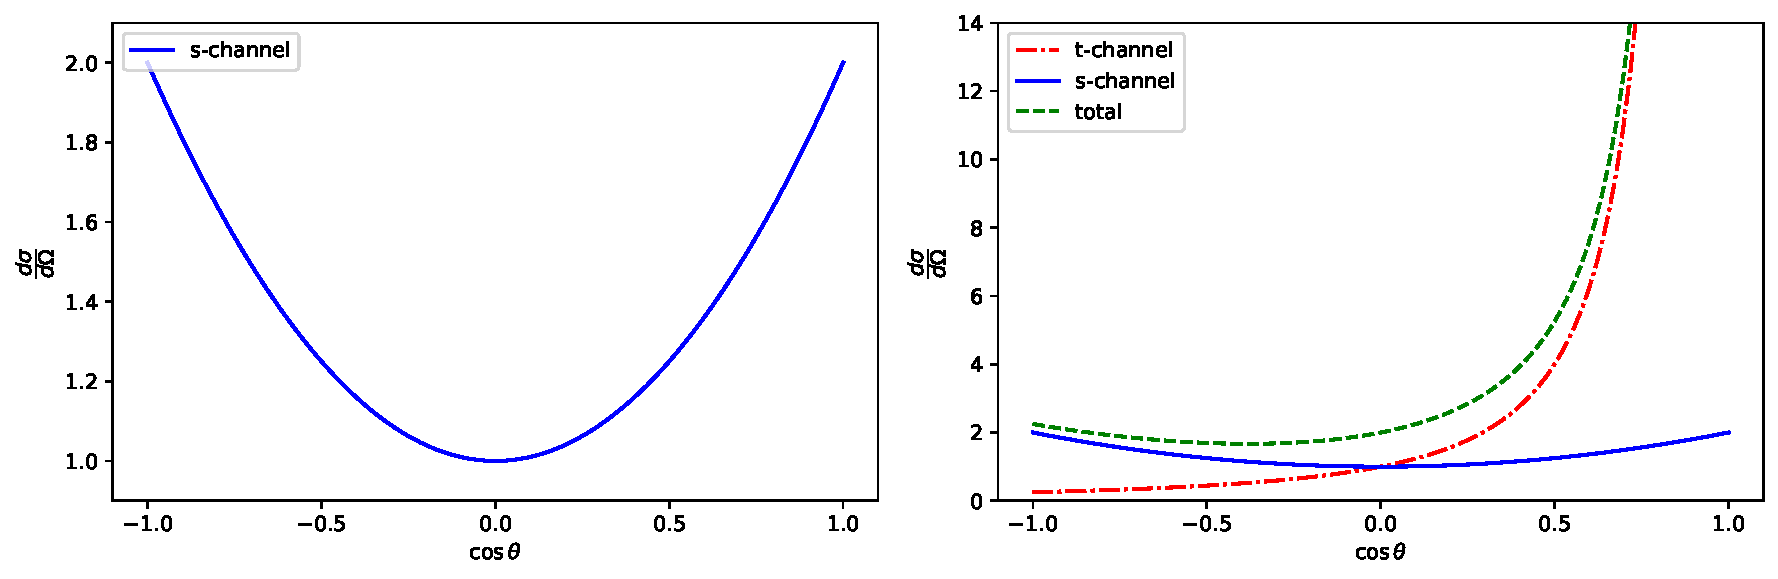
\includegraphics[width=\textwidth]{angulardist.pdf}
\caption[Angular distributions of $e^{+}e^{-}\rightarrow \mu^{+}\mu^{-}$ and $e^{+}e^{-}\rightarrow e^{+}e^{-}$]{Angular distributions of $e^{+}e^{-}\rightarrow \mu^{+}\mu^{-}$ (left) and $e^{+}e^{-}\rightarrow e^{+}e^{-}$ (right)}
\label{angdist}
\end{figure}

\section{Calculation of forward-backward asymmetry}
We are required to calculate the forward-backward asymmetry factor, $A_{FB}$ in the process $e^{+}e^{-}\rightarrow \mu^{+}\mu^{-}$. In order to do this, the following formula is used:
\begin{equation}
A_{FB}=\dfrac{3F_{2}}{4F_{1}}
\end{equation}
where the parameters are given by:
\begin{description}
\item $F_{1}(s)=Q_{f}^{2}-2v_{e}v_{f}Q_{f}\mathfrak{Re}(\chi)+(v_{e}^{2}+a_{e}^{2})(v_{f}^{2}+a_{f}^{2})|\chi|^{2}$
\item $F_{2}(s)=-2a_{e}a_{f}Q_{f}\mathfrak{Re}(\chi)+4v_{e} a_{e} v_{f} a_{f} |\chi|^{2}$
\item $v_{f}=\dfrac{g_{V}^{f}}{2\sin\theta_{W}\cos\theta_{W}}=\dfrac{I_{3}^{f}-2Q_{f}\sin^{2}\theta_{W}}{2\sin\theta_{W}\cos\theta_{W}}$
\item $a_{f}=\dfrac{g_{A}^{f}}{2\sin\theta_{W}\cos\theta_{W}}=\dfrac{I_{3}^{f}}{2\sin\theta_{W}\cos\theta_{W}}$
\item $\chi(s)=\dfrac{s}{\left(\left(s-M_{Z}^{2}\right)+is\dfrac{\Gamma_{Z}}{M_{Z}}\right)}$, Propagator
\item $s$: Square of centre-of-mass energy
\end{description}

The calculated asymmetry factors for various combinations of $\sin^{2}\theta_{W}$ and centre of mass energies, $\sqrt{s}$ are given in Table \ref{fbasymm}.

\begin{table}[h!]
\centering
\begin{tabular}{|c|c|c|c|}
\hline
\diagbox{$\sin^{2}\theta_{W}$}{$\sqrt{s}$ / GeV} & 89.225 & 91.225 & 93.225\\
\hline
0.21 & -0.0937 & 0.0762 & 0.2317\\
\hline
0.23 & -0.1639 & 0.0228 & 0.1965\\
\hline
0.25 & -0.1948 & 0.0042 & 0.1906\\
\hline
\end{tabular}
\caption{Forward backward asymmetry factors for different Weinberg angles ($\theta_{W}$) and centre of mass energies ($\sqrt{s}$)}
\label{fbasymm}
\end{table}